\documentclass{beamer}
\usepackage{epstopdf}
\usepackage{tabularx}
\usepackage{adjustbox}
\usepackage{pdflscape}
\usepackage[]{hyperref}
\definecolor{links}{HTML}{0B610B} % dark green
%\definecolor{links}{HTML}{2A1B81} % dark blue
\hypersetup{colorlinks,linkcolor=,urlcolor=links}
\usepackage{multirow} % for tables
\usepackage{multicol}
\usepackage{subfig}
\usepackage{graphicx}
\usetheme{Madrid}
\title[Hashing classification for tracking ]{Hashing Classification for charged particle tracking}
\author[Luiza Adelina Ciucu (ATLAS) ]{Luiza Adelina Ciucu (ATLAS)} 

\titlegraphic{
%
\includegraphics[height=2.1cm]{./physics_section_EN_q.eps} 

\includegraphics[height=2.1cm]{./physics_section_EN_q-eps-converted-to.pdf} 
}

\date{03 July 2020}

\begin{document}

\frame{\titlepage}

%\texttt{\detokenize{

% define input folder for our plots only once
\newcommand\inputFolderMerge{../output_new_ev_000_100_min_10}
\newcommand\inputFolderMergedBalanced{../output_new_ev_000_100_min_10_balanced17}
\newcommand\inputFolderNN{../output_new_ev_000_100_min_10_NN_07}
\newcommand\inputFolderOverlay{../output_overlay_balanced_ev_000_100_Min10_17}

% add some useful definitions
%\def\MeV{\ifmmode {\mathrm{\ Me\kern -0.1em V}}\else
%                   \textrm{Me\kern -0.1em V}\fi}%  

\def\volumeID{\texttt{\detokenize{volume_id}}}
\def\layerID{\texttt{\detokenize{layer_id}}}

\def\TP{\ifmmode {\mathrm{TP}}\else
                   \textrm{TP}\fi}%
\def\FP{\ifmmode {\mathrm{FP}}\else
                   \textrm{FP}\fi}%                                     
\def\FN{\ifmmode {\mathrm{FN}}\else
                   \textrm{FN}\fi}%
\def\TN{\ifmmode {\mathrm{TN}}\else
                   \textrm{TN}\fi}%

\def\Ni{\ifmmode {\mathrm{N}_\mathrm{i}}\else
                   \textrm{N}_{\textrm{i}}\fi}%
\def\wi{\ifmmode {\mathrm{w}_\mathrm{i}}\else
                   \textrm{w}_{\textrm{i}}\fi}%
\def\xi{\ifmmode {\mathrm{x}_\mathrm{i}}\else
                   \textrm{x}_{\textrm{i}}\fi}%
\def\wzero{\ifmmode {\mathrm{w}_\mathrm{0}}\else
                   \textrm{w}_{\textrm{0}}\fi}%
\def\xzero{\ifmmode {\mathrm{x}_\mathrm{0}}\else
                   \textrm{x}_{\textrm{0}}\fi}%
                   


% intro slide
\begin{frame}{Introduction}
\begin{enumerate}
\item[o] 100 events. For each group of 10: 7 train, 3 test.  
\item[o] If nbPositiveHit$<$10, set nbPositiveHit=0 and output made only of -1.
\item[o] For Train used Balanced (130k), for Test use Unbalanced (3.2M).
\item[o] Balancing Train in two steps, as shown last time.
\begin{enumerate}
\item[-] Make peak flat between 10-17 (with value of 17).
\item[-] Reduce nbPositiveHit=0 until 50\% Pos, 50\% Neg.
\end{enumerate}
\item[o] New studies today
 \begin{enumerate}
\item[-] Last time Test was also Balanced. Now Test is Unbalanced.
\item[-] With constraint of our output of -1 and 1: 
\item[-] Try other output layer activation functions: tanh, squared non linear, soft sign.
\item[-] Try other loss functions: squared hinge and hinge.
\item[-] Try 120 epochs vs 50 epochs.
\end{enumerate}

\end{enumerate}
\end{frame}
\clearpage



\begin{frame}{Balancing method 1/6}
\begin{enumerate}
\item[o] Categories of nbPositiveHit from 0 to 20 denoted $\xi$.
\item[o] Each category has $\Ni$ buckets, representing the weight $\wi$ of $\xi$.
\item[o] The weighted average of nbPositiveHit is desired to be 10, so: \\
$\frac{\wzero \cdot \xzero + \sum_{1}^{20} \wi \cdot \xi}{\wzero + \sum_{1}^{20} \wi}$ = 10
\item[o] Solve for $\wzero$, \\
$\wzero = \frac{ \sum_{1}^{20} \wi \cdot \xi}{10} - \sum_{1}^{20} \wi$
\item[o] Reduce the number of buckets in nbPositiveHit=0 to $\wzero$.
\end{enumerate}
\includegraphics[width=0.49\textwidth]{\inputFolderMergedBalanced_balanced/plot_histo_2_NbBucket_vs_NbPositiveHit_Test.pdf}
\includegraphics[width=0.49\textwidth]{\inputFolderMergedBalanced_balanced/plot_histo_2_NbBucket_vs_NbPositiveHit_normalized_Test.pdf}
\end{frame}
\clearpage

\begin{frame}{Balancing method 2/6}
\begin{enumerate}
\item[o] Positive and Negative hits are now balanced.
\item[o] But we also want as flat as possible distribution to the right.
\item[o] We flatten the peak, so that bins from 10 to N \\ have the nb of buckets as bin N.  
\item[o] Then recalculate nb of buckets for bin 0, as in previous slide.
\item[o] For example, for N=13, \\ where also N=0 gives about the same nb of buckets as N=13. 
\end{enumerate}
\includegraphics[width=0.49\textwidth]{\inputFolderMergedBalanced_balanced13/plot_histo_2_NbBucket_vs_NbPositiveHit_Test.pdf}
\includegraphics[width=0.49\textwidth]{\inputFolderMergedBalanced_balanced13/plot_histo_2_NbBucket_vs_NbPositiveHit_normalized_Test.pdf}
\end{frame}
\clearpage

\begin{frame}{Balancing method 3/6, N=14 and N=15}
\includegraphics[width=0.49\textwidth]{\inputFolderMergedBalanced_balanced14/plot_histo_2_NbBucket_vs_NbPositiveHit_Test.pdf}
\includegraphics[width=0.49\textwidth]{\inputFolderMergedBalanced_balanced14/plot_histo_2_NbBucket_vs_NbPositiveHit_normalized_Test.pdf}\\
\includegraphics[width=0.49\textwidth]{\inputFolderMergedBalanced_balanced15/plot_histo_2_NbBucket_vs_NbPositiveHit_Test.pdf}
\includegraphics[width=0.49\textwidth]{\inputFolderMergedBalanced_balanced15/plot_histo_2_NbBucket_vs_NbPositiveHit_normalized_Test.pdf}
\end{frame}
\clearpage

\begin{frame}{Balancing method 4/6, N=16 and N=17}
\includegraphics[width=0.49\textwidth]{\inputFolderMergedBalanced_balanced16/plot_histo_2_NbBucket_vs_NbPositiveHit_Test.pdf}
\includegraphics[width=0.49\textwidth]{\inputFolderMergedBalanced_balanced16/plot_histo_2_NbBucket_vs_NbPositiveHit_normalized_Test.pdf}\\
\includegraphics[width=0.49\textwidth]{\inputFolderMergedBalanced_balanced17/plot_histo_2_NbBucket_vs_NbPositiveHit_Test.pdf}
\includegraphics[width=0.49\textwidth]{\inputFolderMergedBalanced_balanced17/plot_histo_2_NbBucket_vs_NbPositiveHit_normalized_Test.pdf}
\end{frame}
\clearpage




\begin{frame}{Balancing method 5/6, N=18 and N=19}
\includegraphics[width=0.49\textwidth]{\inputFolderMergedBalanced_balanced18/plot_histo_2_NbBucket_vs_NbPositiveHit_Test.pdf}
\includegraphics[width=0.49\textwidth]{\inputFolderMergedBalanced_balanced18/plot_histo_2_NbBucket_vs_NbPositiveHit_normalized_Test.pdf}\\
\includegraphics[width=0.49\textwidth]{\inputFolderMergedBalanced_balanced19/plot_histo_2_NbBucket_vs_NbPositiveHit_Test.pdf}
\includegraphics[width=0.49\textwidth]{\inputFolderMergedBalanced_balanced19/plot_histo_2_NbBucket_vs_NbPositiveHit_normalized_Test.pdf}
\end{frame}
\clearpage



\begin{frame}{Balancing method 6/6, N=20, and Table for Train.}
\includegraphics[width=0.49\textwidth]{\inputFolderMergedBalanced_balanced20/plot_histo_2_NbBucket_vs_NbPositiveHit_Test.pdf}
\includegraphics[width=0.49\textwidth]{\inputFolderMergedBalanced_balanced20/plot_histo_2_NbBucket_vs_NbPositiveHit_normalized_Test.pdf}
\begin{table}[ht]
\centering
\resizebox{\textwidth}{!}{\begin{tabular}{|l|l|l|l|l|l|}
\hline
Max bin of flat peak & nbBucket Total & nbBucket bin 0 & nbBucket peak & \% bin 0 & \% peak \\ \hline
13 & 2021k & 362k & 324k & 17.9 &16.0 \\ \hline
14 & 1510k &  296k & 213k & 19.6 & 14.1 \\ \hline
15 & 0805k & 178k & 096k & 22.1 &11.9 \\ \hline
16 & 0345k & 086k & 034k & 24.9 &10.0 \\ \hline
17 & 0130k & 036k & 011k & 28.0 & 08.3 \\ \hline
18 &0074k & 022k & 006k & 29.6& 07.7 \\ \hline
19 & 0022k & 007k & 001k & 32.1& 06.5 \\ \hline
20 & 0019k & 003k & 001k & 33.3 & 06.1\\ \hline 
\hline
\end{tabular}}
\caption{Caption} 
\end{table} 
\end{frame}
\clearpage

\begin{frame}{Accuracy and Loss from training}
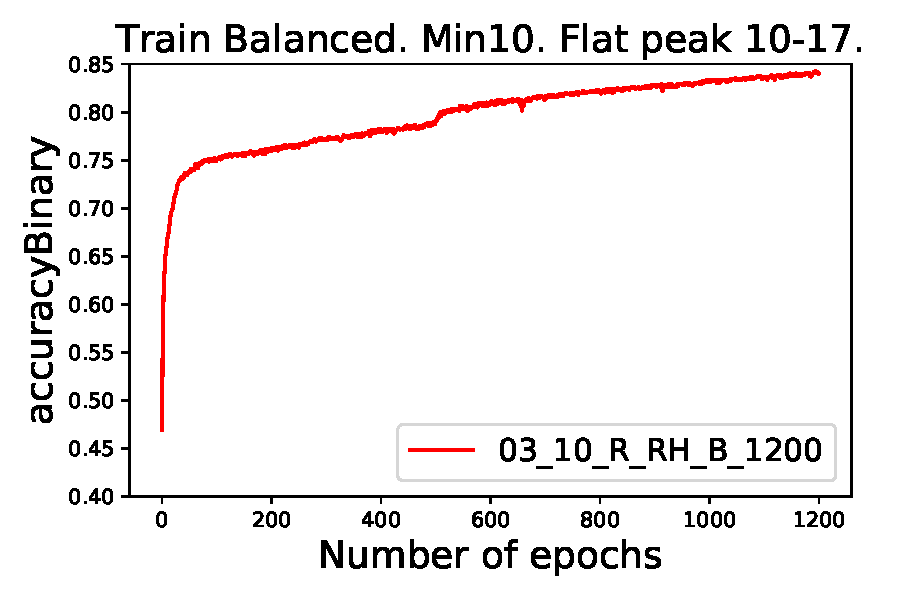
\includegraphics[width=0.49\textwidth]{\inputFolderOverlay/plot_01_1_overlay_graph_accuracyBinary_Train.pdf}
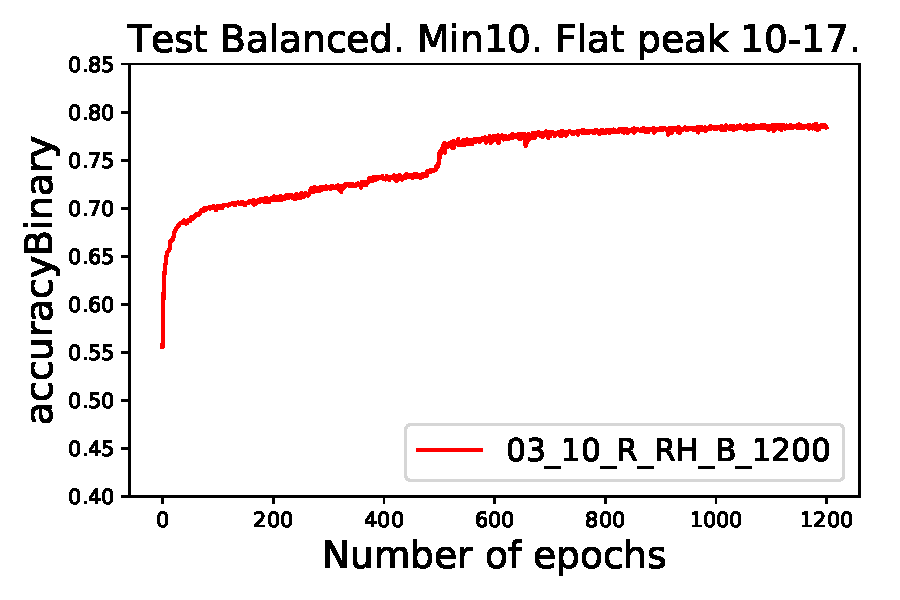
\includegraphics[width=0.49\textwidth]{\inputFolderOverlay/plot_01_1_overlay_graph_accuracyBinary_Test.pdf}\\
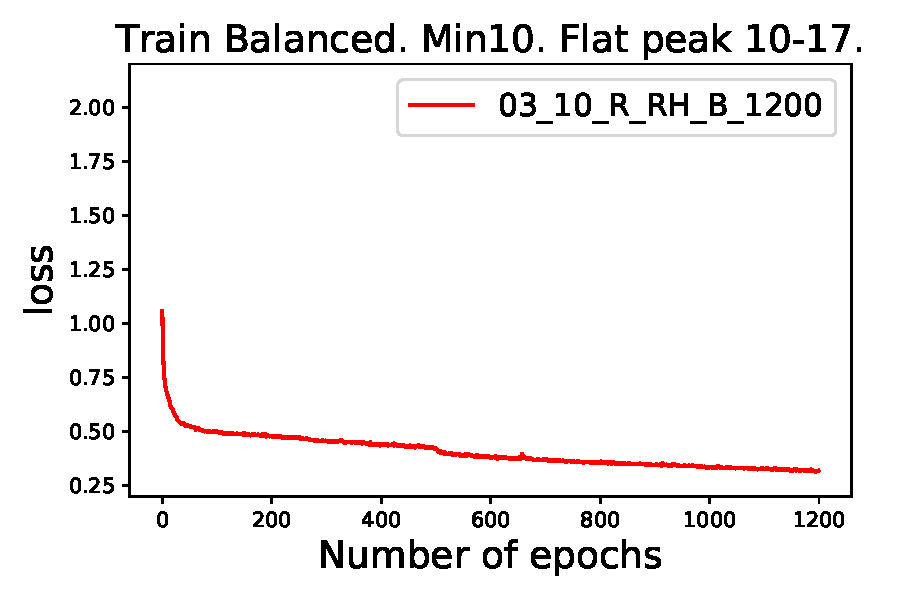
\includegraphics[width=0.49\textwidth]{\inputFolderOverlay/plot_01_1_overlay_graph_loss_Train.pdf}
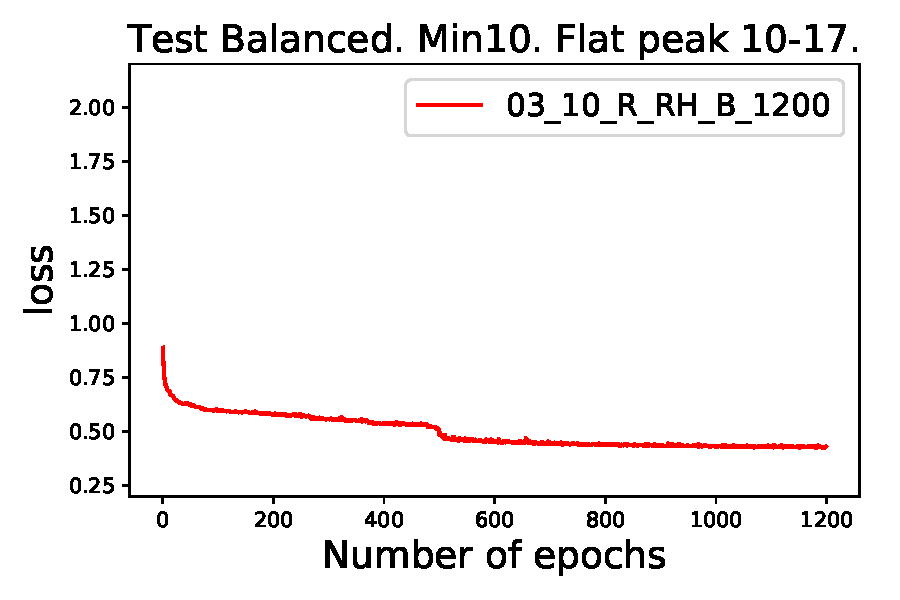
\includegraphics[width=0.49\textwidth]{\inputFolderOverlay/plot_01_1_overlay_graph_loss_Test.pdf}
\end{frame}
\clearpage

\begin{frame}{Metrics for each VolumeID overlay balancing methods.}
\begin{enumerate}
\item[o] If unbalanced, as seen before, precision and recall were zero, as it learned to predict all buckets with negative hits.
\item[o] Now in all methods of balancing, precision and recall are not zero.
\item[o] Best performance seems when the peak is most flat, so for 19 and 20. 
\item[o] 19 and 20 have also very few buckets remaining, so fast to process.
\end{enumerate}
\centering
% table
\begin{center}
\begin{tabular}{ |c|c|c| } 
\hline
Accuracy & Precision & Recall \\ 
\hline
$\frac{\TP+\TN}{\TP+\FP+\FN+\TN}$ & $\frac{\TP}{\TP+\FP}$  & $\frac{\TP}{\TP+\FN}$ \\ 
\hline
\end{tabular}
\end{center}
% plots
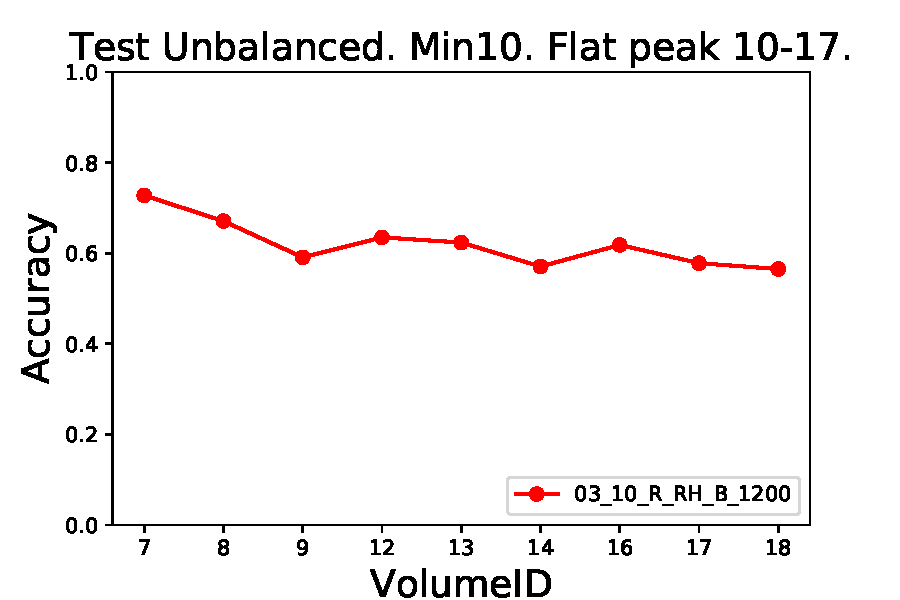
\includegraphics[width=0.32\textwidth]{\inputFolderOverlay/plot_03_1_overlay_graph_Accuracy_VolumeID_Test.pdf}
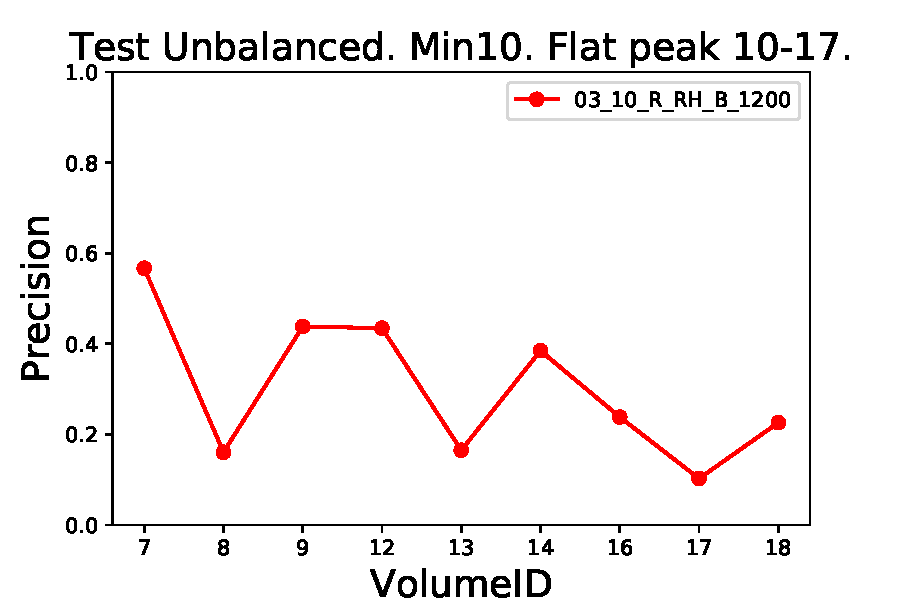
\includegraphics[width=0.32\textwidth]{\inputFolderOverlay/plot_03_1_overlay_graph_Precision_VolumeID_Test.pdf}
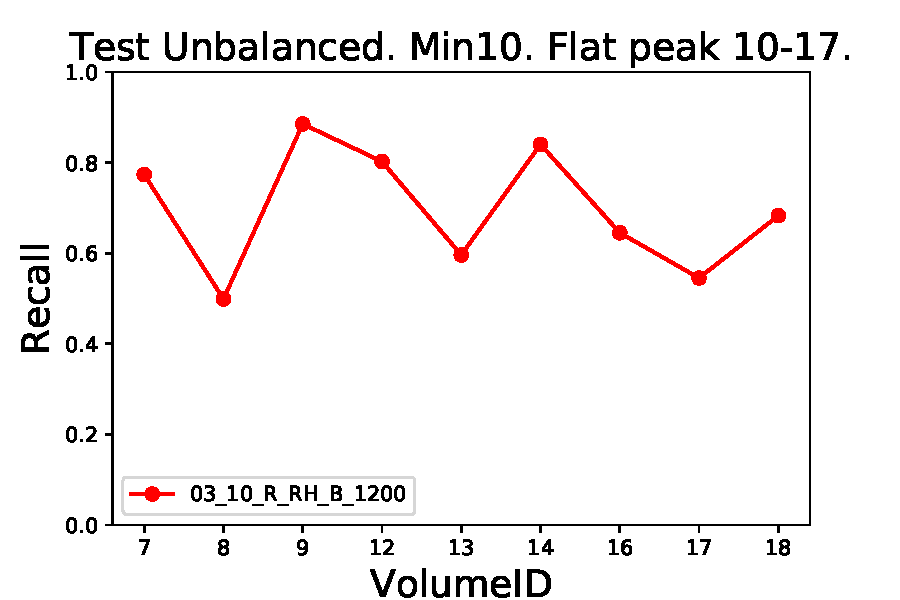
\includegraphics[width=0.32\textwidth]{\inputFolderOverlay/plot_03_1_overlay_graph_Recall_VolumeID_Test.pdf}\\
\end{frame}

\begin{frame}{2D plots Balanced no flat peak}
\includegraphics[width=0.49\textwidth]{\inputFolderMergedBalanced_NN/NN_5_Balanced_120_50000_histo_OutputPositive.pdf}
\includegraphics[width=0.49\textwidth]{\inputFolderMergedBalanced_NN/NN_5_Balanced_120_50000_histo_PredictedOutputPositive.pdf}\\
\includegraphics[width=0.49\textwidth]{\inputFolderMergedBalanced_NN/NN_5_Balanced_120_50000_histo_OutputPositive_vs_PredictedOutputPositive_Train.pdf}
\includegraphics[width=0.49\textwidth]{\inputFolderMergedBalanced_NN/NN_5_Balanced_120_50000_histo_OutputPositive_vs_PredictedOutputPositive_Test.pdf}
\end{frame}
\clearpage

\begin{frame}{2D plots Balanced flat peak 10-13}
\includegraphics[width=0.49\textwidth]{\inputFolderMergedBalanced_NN/NN_5_Balanced13_120_50000_histo_OutputPositive.pdf}
\includegraphics[width=0.49\textwidth]{\inputFolderMergedBalanced_NN/NN_5_Balanced13_120_50000_histo_PredictedOutputPositive.pdf}\\
\includegraphics[width=0.49\textwidth]{\inputFolderMergedBalanced_NN/NN_5_Balanced13_120_50000_histo_OutputPositive_vs_PredictedOutputPositive_Train.pdf}
\includegraphics[width=0.49\textwidth]{\inputFolderMergedBalanced_NN/NN_5_Balanced13_120_50000_histo_OutputPositive_vs_PredictedOutputPositive_Test.pdf}
\end{frame}
\clearpage

\begin{frame}{2D plots Balanced flat peak 10-14}
\includegraphics[width=0.49\textwidth]{\inputFolderMergedBalanced_NN/NN_5_Balanced14_120_50000_histo_OutputPositive.pdf}
\includegraphics[width=0.49\textwidth]{\inputFolderMergedBalanced_NN/NN_5_Balanced14_120_50000_histo_PredictedOutputPositive.pdf}\\
\includegraphics[width=0.49\textwidth]{\inputFolderMergedBalanced_NN/NN_5_Balanced14_120_50000_histo_OutputPositive_vs_PredictedOutputPositive_Train.pdf}
\includegraphics[width=0.49\textwidth]{\inputFolderMergedBalanced_NN/NN_5_Balanced14_120_50000_histo_OutputPositive_vs_PredictedOutputPositive_Test.pdf}
\end{frame}
\clearpage

\begin{frame}{2D plots Balanced flat peak 10-15}
\includegraphics[width=0.49\textwidth]{\inputFolderMergedBalanced_NN/NN_5_Balanced15_120_50000_histo_OutputPositive.pdf}
\includegraphics[width=0.49\textwidth]{\inputFolderMergedBalanced_NN/NN_5_Balanced15_120_50000_histo_PredictedOutputPositive.pdf}\\
\includegraphics[width=0.49\textwidth]{\inputFolderMergedBalanced_NN/NN_5_Balanced15_120_50000_histo_OutputPositive_vs_PredictedOutputPositive_Train.pdf}
\includegraphics[width=0.49\textwidth]{\inputFolderMergedBalanced_NN/NN_5_Balanced15_120_50000_histo_OutputPositive_vs_PredictedOutputPositive_Test.pdf}
\end{frame}
\clearpage

\begin{frame}{2D plots Balanced flat peak 10-16}
\includegraphics[width=0.49\textwidth]{\inputFolderMergedBalanced_NN/NN_5_Balanced16_120_50000_histo_OutputPositive.pdf}
\includegraphics[width=0.49\textwidth]{\inputFolderMergedBalanced_NN/NN_5_Balanced16_120_50000_histo_PredictedOutputPositive.pdf}\\
\includegraphics[width=0.49\textwidth]{\inputFolderMergedBalanced_NN/NN_5_Balanced16_120_50000_histo_OutputPositive_vs_PredictedOutputPositive_Train.pdf}
\includegraphics[width=0.49\textwidth]{\inputFolderMergedBalanced_NN/NN_5_Balanced16_120_50000_histo_OutputPositive_vs_PredictedOutputPositive_Test.pdf}
\end{frame}
\clearpage

\begin{frame}{2D plots Balanced flat peak 10-17}
\includegraphics[width=0.49\textwidth]{\inputFolderMergedBalanced_NN/NN_5_Balanced17_120_50000_histo_OutputPositive.pdf}
\includegraphics[width=0.49\textwidth]{\inputFolderMergedBalanced_NN/NN_5_Balanced17_120_50000_histo_PredictedOutputPositive.pdf}\\
\includegraphics[width=0.49\textwidth]{\inputFolderMergedBalanced_NN/NN_5_Balanced17_120_50000_histo_OutputPositive_vs_PredictedOutputPositive_Train.pdf}
\includegraphics[width=0.49\textwidth]{\inputFolderMergedBalanced_NN/NN_5_Balanced17_120_50000_histo_OutputPositive_vs_PredictedOutputPositive_Test.pdf}
\end{frame}
\clearpage

\begin{frame}{2D plots Balanced flat peak 10-18}
\includegraphics[width=0.49\textwidth]{\inputFolderMergedBalanced_NN/NN_5_Balanced18_120_50000_histo_OutputPositive.pdf}
\includegraphics[width=0.49\textwidth]{\inputFolderMergedBalanced_NN/NN_5_Balanced18_120_50000_histo_PredictedOutputPositive.pdf}\\
\includegraphics[width=0.49\textwidth]{\inputFolderMergedBalanced_NN/NN_5_Balanced18_120_50000_histo_OutputPositive_vs_PredictedOutputPositive_Train.pdf}
\includegraphics[width=0.49\textwidth]{\inputFolderMergedBalanced_NN/NN_5_Balanced18_120_50000_histo_OutputPositive_vs_PredictedOutputPositive_Test.pdf}
\end{frame}
\clearpage

\begin{frame}{2D plots Balanced flat peak 10-19}
\includegraphics[width=0.49\textwidth]{\inputFolderMergedBalanced_NN/NN_5_Balanced19_120_50000_histo_OutputPositive.pdf}
\includegraphics[width=0.49\textwidth]{\inputFolderMergedBalanced_NN/NN_5_Balanced19_120_50000_histo_PredictedOutputPositive.pdf}\\
\includegraphics[width=0.49\textwidth]{\inputFolderMergedBalanced_NN/NN_5_Balanced19_120_50000_histo_OutputPositive_vs_PredictedOutputPositive_Train.pdf}
\includegraphics[width=0.49\textwidth]{\inputFolderMergedBalanced_NN/NN_5_Balanced19_120_50000_histo_OutputPositive_vs_PredictedOutputPositive_Test.pdf}
\end{frame}
\clearpage

\begin{frame}{2D plots Balanced flat peak 10-20}
\includegraphics[width=0.49\textwidth]{\inputFolderMergedBalanced_NN/NN_5_Balanced20_120_50000_histo_OutputPositive.pdf}
\includegraphics[width=0.49\textwidth]{\inputFolderMergedBalanced_NN/NN_5_Balanced20_120_50000_histo_PredictedOutputPositive.pdf}\\
\includegraphics[width=0.49\textwidth]{\inputFolderMergedBalanced_NN/NN_5_Balanced20_120_50000_histo_OutputPositive_vs_PredictedOutputPositive_Train.pdf}
\includegraphics[width=0.49\textwidth]{\inputFolderMergedBalanced_NN/NN_5_Balanced20_120_50000_histo_OutputPositive_vs_PredictedOutputPositive_Test.pdf}
\end{frame}
\clearpage

\begin{frame}{Conclusion}
\begin{enumerate}
\item[o] 100 events, 70 in train, 30 in test.
\item[o] If nbPositiveHit$<$10, set nbPositiveHit=0 and output made only of -1.
\item[o] Balanced nb positive and negative hits by reducing the number of buckets at bin 0, with no flat peak or with various lengths of flat peak.
\item[o] Best accuracy, precision and recall for 19-20.
\item[o] But closest PredictedOutputPositive to OutputPositive for 16-17.
\item[o] Overall best choice seems with flat peak between 10 and 17, then rebalance at bin 0. 
\item[o] Next steps: write thesis.
\end{enumerate}
\end{frame}
\clearpage

\end{document}
